%Fig~\ref{fig:Figure_2} %
%% Copyright 2022 OXFORD UNIVERSITY PRESS
%%
%% This file is part of the 'oup-authoring-template Bundle'.
%% ---------------------------------------------
%%
%% It may be distributed under the conditions of the LaTeX Project Public
%% License, either version 1.2 of this license or (at your option) any
%% later version.  The latest version of this license is in
%%    http://www.latex-project.org/lppl.txt
%% and version 1.2 or later is part of all distributions of LaTeX
%% version 1999/12/01 or later.
%%
%% The list of all files belonging to the 'oup-authoring-template Bundle' is
%% given in the file `manifest.txt'.
%%
%% Template article for OXFORD UNIVERSITY PRESS's document class `oup-authoring-template'
%% with bibliographic references
%%

%%%CONTEMPORARY%%%
%\documentclass[unnumsec,webpdf,contemporary,large]{oup-authoring-template}%
\documentclass[unnumsec,webpdf,contemporary,large,namedate]{oup-authoring-template}% uncomment this line for author year citations and comment the above
%\documentclass[unnumsec,webpdf,contemporary,medium]{oup-authoring-template}
%\documentclass[unnumsec,webpdf,contemporary,small]{oup-authoring-template}

%%%MODERN%%%
%\documentclass[unnumsec,webpdf,modern,large]{oup-authoring-template}
%\documentclass[unnumsec,webpdf,modern,large,namedate]{oup-authoring-template}% uncomment this line for author year citations and comment the above
%\documentclass[unnumsec,webpdf,modern,medium]{oup-authoring-template}
%\documentclass[unnumsec,webpdf,modern,small]{oup-authoring-template}

%%%TRADITIONAL%%%
%\documentclass[unnumsec,webpdf,traditional,large]{oup-authoring-template}
%\documentclass[unnumsec,webpdf,traditional,large,namedate]{oup-authoring-template}% uncomment this line for author year citations and comment the above
%\documentclass[unnumsec,namedate,webpdf,traditional,medium]{oup-authoring-template}
%\documentclass[namedate,webpdf,traditional,small]{oup-authoring-template}

%\onecolumn % for one column layouts

%\usepackage{showframe}

\graphicspath{{Fig/}}

% line numbers
%\usepackage[mathlines, switch]{lineno}
%\usepackage[right]{lineno}
\usepackage{hyperref}
\usepackage{lmodern}
%\usepackage{graphicx}
%\usepackage{xr}

\begin{document}

\journaltitle{Bioinformatics}
\journaltitle{Preprint}
\DOI{DOI HERE}
\copyrightyear{2024}
% \pubyear{2019}
% \access{Advance Access Publication Date: Day Month Year}
\appnotes{Paper}

\firstpage{1}

\title[tsbrowse]{Tsbrowse: a genome browser for Ancestral Recombination Graphs}

\author[1$\ast$]{Savita Karthikeyan}
\author[1]{Ben Jeffery}
\author[1]{Duncan Mbuli-Robertson}
\author[1]{Jerome Kelleher \ORCID{0000-0000-0000-0000}}

\authormark{Karthikeyan et al.}

\address[1]{\orgdiv{Big Data Institute, Li Ka Shing Centre for Health
        Information and Discovery}, \orgname{University of Oxford},
    \orgaddress{\street{Old Road Campus}, \postcode{Oxford OX3 7LF},
        \country{United Kingdom}}}

\corresp[$\ast$]{Corresponding author.
    \href{email:savita.karthikeyan@st-hughs.ox.ac.uk}{savita.karthikeyan@st-hughs.ox.ac.uk}}

\received{Date}{0}{Year}
\revised{Date}{0}{Year}
\accepted{Date}{0}{Year}

\abstract{
    %\textbf{Motivation:}
    Ancestral Recombination Graphs (ARGs) represent the interwoven paths of genetic
    ancestry for a set of recombining sequences. The ability to capture the
    evolutionary history of samples makes ARGs valuable in a wide range of
    applications in population and statistical genetics. ARG-based approaches are
    increasingly becoming a part of genetic data analysis pipelines due to
    breakthroughs enabling ARG inference at biobank-scale. However, there is a lack
    of visualisation tools, which are crucial for validating inferences and
    generating hypotheses.
    %\textbf{Results:} 
    We present \texttt{tsbrowse}, an open-source Python web-app for the interactive
    visualisation of the fundamental building-blocks of ARGs, i.e.,  nodes, edges
    and mutations. We demonstrate the application of \texttt{tsbrowse} to various
    data sources and scenarios, and highlight its key features of browsability
    along the genome, user interactivity, and scalability to very large sample
    sizes.\\ \textbf{Availability:}\\ Python package:
    \texttt{\url{https://pypi.org/project/tsbrowse/}}, \\ Development version:
    \texttt{\url{https://github.com/tskit.dev/tsbrowse}}, \\ Documentation:
    \texttt{\url{https://tskit.dev/tsbrowse/docs/}}\\
    %\textbf{Contact:} \href{name@email.com}{name@email.com}\\
    %\textbf{Supplementary information:} Available at
    %\textit{\textcolor{red}{\href{https://www.google.com}{Bioinformatics}
    %online}.}}
}

\keywords{Ancestral Recombination Graphs, Holoviz, biobank-scale ARG
    visualisation, genome browser} \maketitle

\section{Introduction}
Ancestral recombination graphs (ARGs) describe how a set of sample
sequences relate to each other at each position along the genome in a
recombining
species, and are currently the subject of intense research
interest~\citep{brandt2024promise,lewanski2024era,nielsen2024inference,
    wong2024general}. ARGs are a fundamental object in population genetics,
and although they have been of theoretical interest for
decades~\citep{Hudson1983,Griffiths1997} it is only with recent breakthroughs
in inference methods~\citep{rasmussen2014genome,
    speidel2019method,kelleher2019inferring,wohns2022unified,zhang2023biobank,
    gunnarsson2024scalable,deng2024robust} that practical application has
become possible. Varied applications have been recently proposed,
such as inferring selection~\citep{stern2019approximate,hejase2022deep} and
the spatial location of genetic ancestors~\citep{osmond2024estimating,deraje2024inferring,grundler2024geographic},
more powerful approaches to quantifying genetic
relatedness~\citep{fan2022genealogical,zhang2023biobank,gunnarsson2024scalable,lehmann2025on}
and other methodological improvements for genome wide association
studies~\citep{nowbandegani2023extremely,link2023tree},
and the development of machine learning methods using inferred
ARGs as input~\citep{hejase2022deep,pearson2023local,korfmann2024simultaneous,
whitehouse2024tree}.
While these developements are exciting, the performance 
of these new methods depends critically on the accuracy of the inferred ARGs.
Although studies benchmarking the various inference methods on 
simulated data have emerged 
\citep{brandt2022evaluation,deng2024robust,peng2024evaluating},
the practicalities of applying ARG inference to real data is 
understudied. In particular, there is a critical lack of software 
infrastructure to support evaluation and quality control of 
inferred ARGs.

Visualisation is fundamentally important to data analysis.
Many specialised tools exist to aid the visual analysis and
quality control
of genome assembly~\citep{wick2015bandage,challis2020blobtoolkit},
read mapping~\citep{robinson2011integrative},
and variant
calling~\citep{robinson2017variant,tollefson2019viva,konig2023divbrowse},
for example.
At every stage of a bioinformatics pipeline, it is important to visualise
results to avoid artefacts and aid understanding of the data.
Genome browsers such as IGV~\citep{robinson2011integrative} and the
UCSC Genome Browser~\citep{nassar2023ucsc} integrate many different
data modalities, and are vital infrastructure for the field.
% . In the past few decades,
% genome browsers have become synonymous with sequence visualisation, by
% providing user-friendly, interactive interfaces to navigate genomic sequences
% and annotations. From early standalone tools to manage \textit{C. elegans} data
% \citep{Eeckman1995}, to modern web-apps for vertebrate genomes
% \citep{Birney2004,Rangwala2024,Nassar2023}, browsers have continued to evolve
% with the changing landscape of genomics. Modern genome browsers can load
% datasets from a URL or local file system \citep{Lee2013,Robinson2023}.
% The data security and scalability offered by this architecture ensures that
% genome browsers continue to be relevant in the biobank era.

There is currently no straightforward means of visually summarising
ARGs, presenting a significant stumbling block for the nascent
field of practical ARG inference. Inferred ARGs are essentially opaque,
with only the most basic numerical summaries (such as numbers
of nodes, mutations etc) or high-level
statistics~\citep{ralph2020efficiently} available. While tools
for visualising the local tree topologies exist, they are difficult
to interpret and do not scale well to large sample sizes.
To address this gap, we present \texttt{tsbrowse}, a
% I worry that if we say "genome browser" we'll get stung for not having 
% deep integration with all sorts of stuff
client-server application providing genome browser-like
functionality for ARGs.
It provides interactive visualisations of the information structure
of ARGs, smoothly scrolling from chromosome-level views down to
individual nodes, edges and mutations. Supporting very large ARGs is a
particular focus for \texttt{tsbrowse}, as millions of genome
sequences have been sampled for several
species~\citep{cesarani2022multibreed,stark2024call,hunt2024addressing}
and ARGs of this scale are a particular focus of ongoing
research~\citep{kelleher2019inferring,zhang2023biobank,
    zhan2023towards,anderson2023on,gunnarsson2024scalable}.

% \citep{Kelleher2019,Speidel2019,Zhang2023,Gunnarsson2024.08.31.610248,Deng2024.03.16.585351}.

% widely-used library for interchanging ARGs inferred using a variety of methods
% \citep{Speidel2019,Zhang2023,Haller2019,Baumdicker2021,Gunnarsson2024.08.31.610248,Deng2024.03.16.585351}.

% The interface is run on a web browser. It works on biobank-scale datasets
% without requiring \textcolor{red}{raw data uploads to a server}. This is ideal
% for performing quality control and exploratory analyses on ARGs inferred from
% biobank datasets. 

\section{Results}

\begin{figure} \centering
    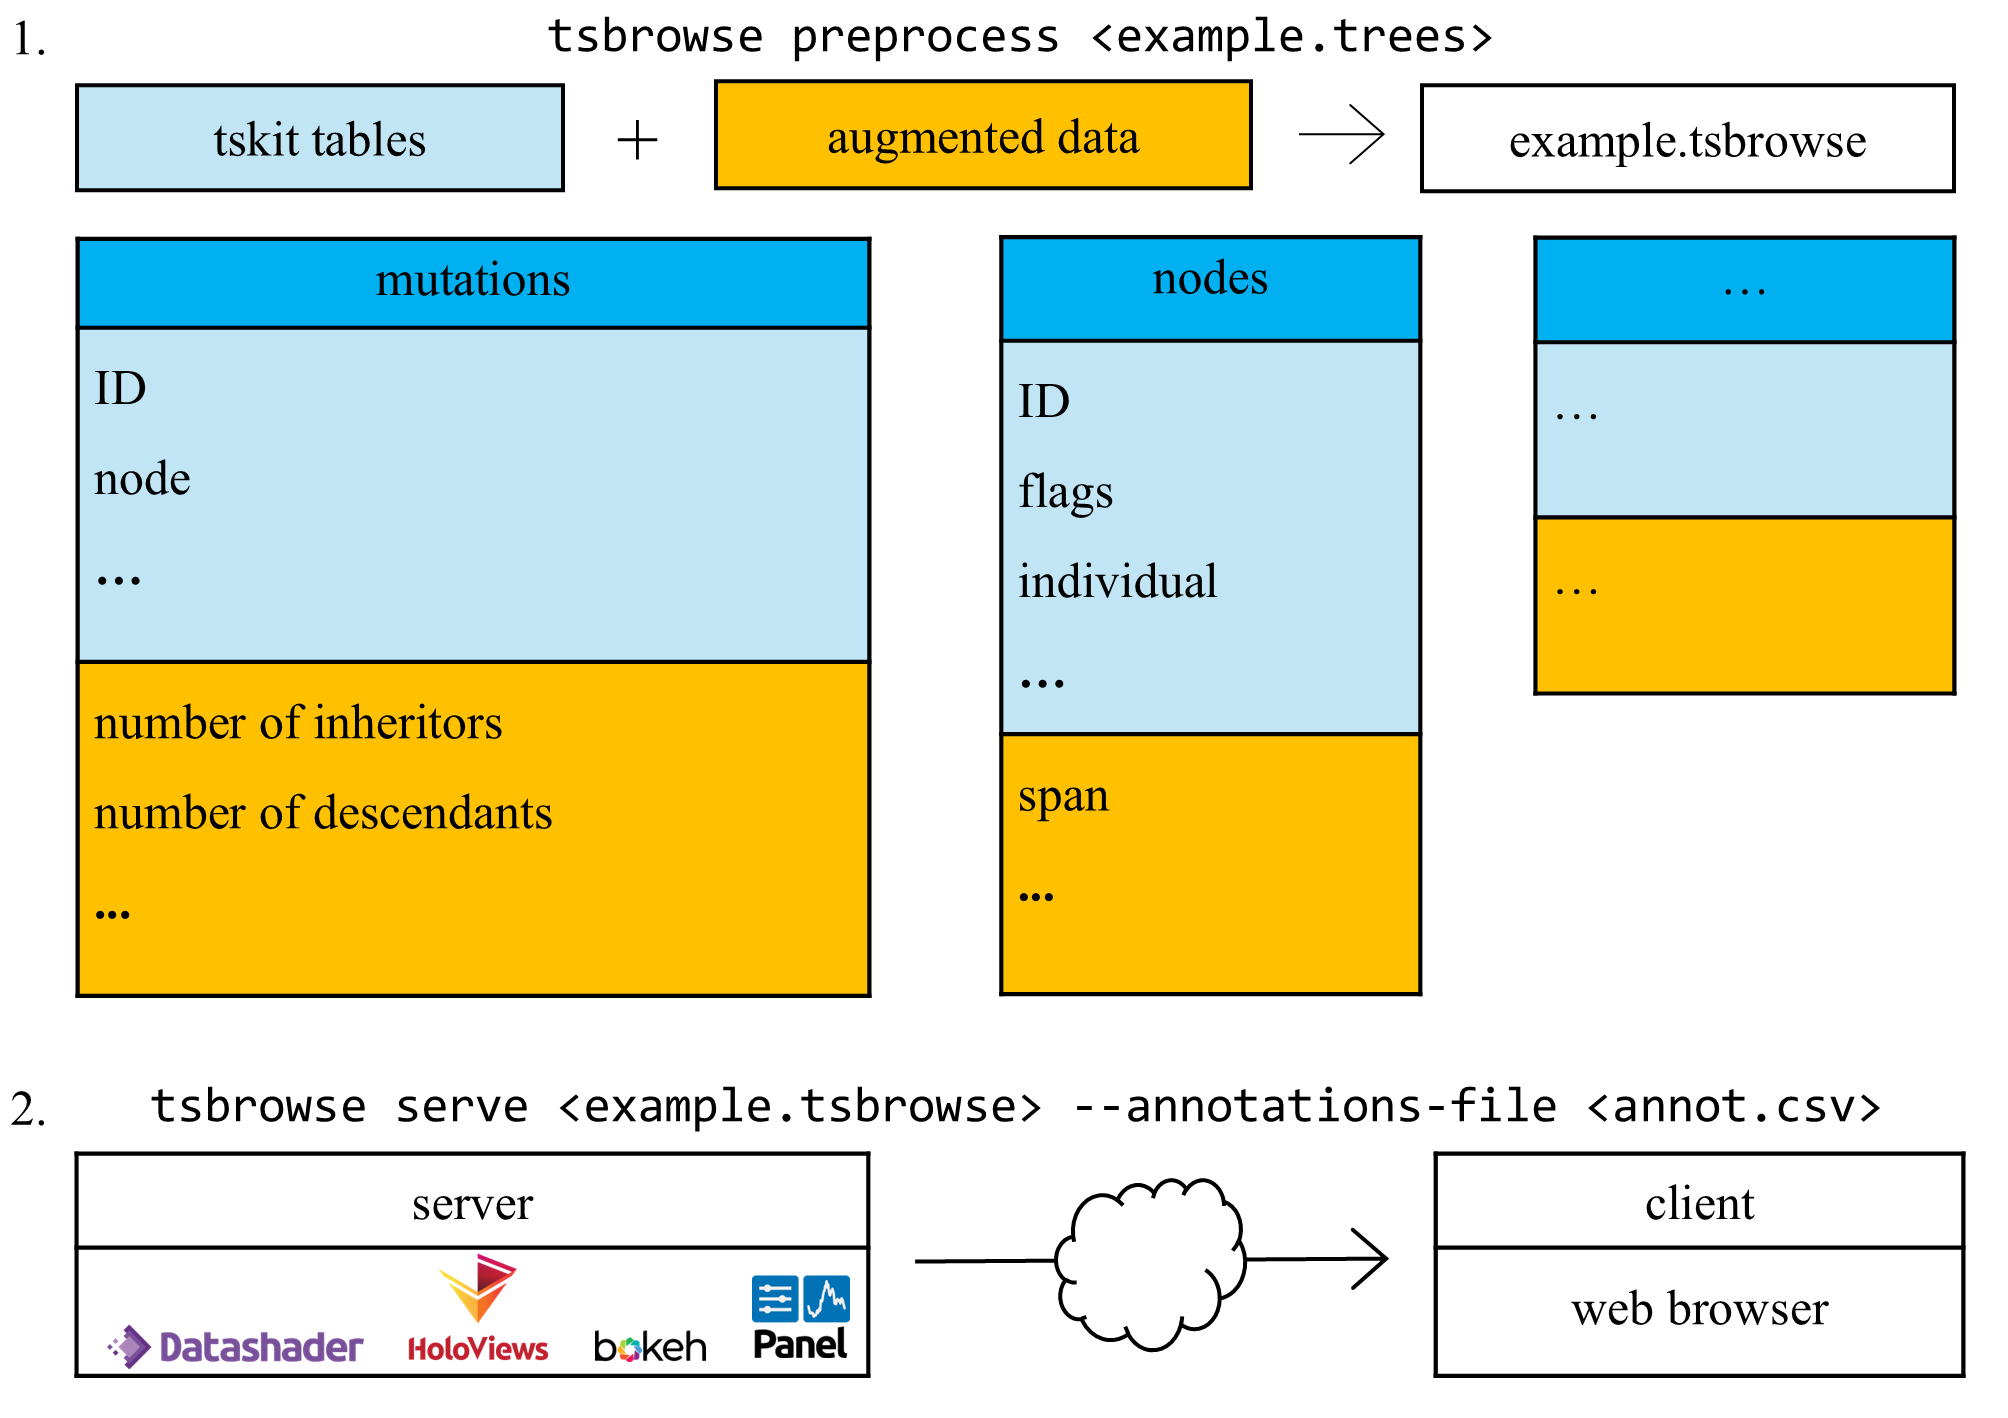
\includegraphics[width=0.95\linewidth]{figures/MainFig1.png}
    \caption{\textbf{Overview of tsbrowse architecture. } In tskit, ARGs are
        defined by a collection of tables. Exemplar
        table names are denoted in dark blue and columns that describe the property in
        light blue. In the pre-process step, tables are augmented with additional
        information computed for each property (yellow). The output from this
        pre-processing step is stored as a \texttt{.tsbrowse} file. Next the serve step
        renders the visualisation in a web browser by leveraging tools in the Holoviz
        ecosystem. Optional annotations are provided as an input file, allowing users
        to overlay contextual information about genes or other sequence features. }
    \label{fig:Figure_1} \end{figure}

\subsection{Data model} \label{subsec:Data_Model} 
\texttt{Tsbrowse} uses the ``succinct tree sequence'' encoding of 
ARGs~\citep{wong2024general}. This efficient ARG encoding 
is implemented by the 
\texttt{tskit} library~\citep{ralph2020efficiently}
and supported by most modern ARG
simulation~\citep{kelleher2016efficient,kelleher2018efficient,
    haller2019tree,baumdicker2022efficient,
    adrion2020community,lauterbur2023expanding,korfmann2023weak,
    tsambos2023link,tagami2024tstrait},
inference~\citep{kelleher2019inferring,speidel2019method,wohns2022unified,
    mahmoudi2022bayesian,zhan2023towards,zhang2023biobank,deng2025general},
and processing methods~\citep{fan2022genealogical,nowbandegani2023extremely}.
In \texttt{tskit}, ARGs are encoded as a
collection of tables, storing information about the
nodes and edges that describe the graph topology and the sites
and mutations that encode the sequence variation (Fig.~\ref{fig:Figure_1}).
% For example, the Node table describes sampled or ancestral sequences
% and records their time of birth, and the individual and population they belong
% to. The Edge table describes the relationship between pairs of nodes, and
% records the node IDs and the genomic locations over which the edge spans. The
% Mutation table records mutation events in the history of the sample, including
% the change of allelic state, time of event and node in which the event
% occurred. 
% The Node and Edge tables describe the genealogical relationships
% between the sampled and ancestral sequences, 
% while the Mutation table describes
% sequence variation contained in the samples. 
% (see \hyperref[subsec:User_Interface]{User Interface}). 

\subsection{Architecture}
\texttt{Tsbrowse} is a modular client-server application
written in Python, optimised for ARGs with millions
of samples (Fig.~\ref{fig:Figure_1}).
The application has two basic commands: \texttt{preprocess}
and \texttt{serve}. The \texttt{preprocess} command
takes an input ARG file and augments the \texttt{tskit}
tables with additional columns,
precomputing all the information required for visualisation,
and storing as a compressed \texttt{.tsbrowse} file.
(The \texttt{.tsbrowse} file is also a valid input for
\texttt{tszip}, a general utility for compressing \texttt{tskit}
files.)
To visualise an ARG we then run \texttt{tsbrowse serve}, which
by default will open a browser window on the local machine, but
also supports running the server on a remote machine across the
network.
This client-server architecture has some important advantages over
a monolithic single-machine approach. Most importantly,
the ARG being visualised remains in-situ and does not need to be
downloaded from the server.

The goal of \texttt{tsbrowse} is to provide interpretable
and interactive visual summaries of ARGs containing millions of nodes, edges
and mutations. Mutations, for example, have a clear interpretation
when plotted on genome coordinate vs time axes, but at this scale
the data density is far too high to simply plot each mutation as a point.
We overcome this problem by using Datashader and the wider
Holoviz ecosystem~\citep{Holoviz}, which efficiently rasterises large datasets
at the requested resolution on the server, sends the image to the web-browser
for display, and dynamically updates as the user interactively navigates the
ARG.
This approach allows us to summarise very large ARGs interactively;
Fig~\ref{fig:Supplementary_Figure_4}, for example, shows a screenshot of
\texttt{tsbrowse} summarising the 1.9 million mutations in a SARS-CoV-2
ARG with around 2.7 million nodes and edges.

% Fig~\ref{fig:Figure_2} shows an example of how edges are visualised 
% under this 

% and renders visualisations. This step follows a client-server architecture. On
% the server side (the machine on which \texttt{tsbrowse serve} is run), the
% Holoviz suite of libraries \citep{Holoviz} is leveraged to create
% visualisations based on the pre-processed data. This choice of architecture is
% prompted by the need to represent properties of large-scale ARGs in a
% meaningful and performant way. For example, a visual representation of millions
% of mutations in SARS-Cov-2 ARGs \citep{zhan2023towards} could quickly
% lead to performance bottlenecks and overplotting. Datashader
% \citep{Datashader}, a component Holoviz package, overcomes this challenge by
% rasterising huge datasets (see \hyperref[subsec:User_Interface]{User Interface}
% for details, and Supplementary Figure \ref{fig:Supplementary_Figure_4} for a
% tsbrowse view of SARS-Cov-2 mutations). A web browser client connects to the

% \texttt{Tsbrowse} is run in a step-wise approach (Fig.~\ref{fig:Figure_1}), 
% which makes it convenient to handle large datasets. 
% The initial step (\texttt{tsbrowse
% preprocess}) prepares the data for visualisation. It can be performed
% separately on a large machine, and the output stored for later use. The second
% step (\texttt{tsbrowse serve}), which can be run on a smaller machine, creates
% and renders visualisations. This step follows a client-server architecture. On
% the server side (the machine on which \texttt{tsbrowse serve} is run), the
% Holoviz suite of libraries \citep{Holoviz} is leveraged to create
% visualisations based on the pre-processed data. This choice of architecture is
% prompted by the need to represent properties of large-scale ARGs in a
% meaningful and performant way. For example, a visual representation of millions
% of mutations in SARS-Cov-2 ARGs \citep{zhan2023towards} could quickly
% lead to performance bottlenecks and overplotting. Datashader
% \citep{Datashader}, a component Holoviz package, overcomes this challenge by
% rasterising huge datasets (see \hyperref[subsec:User_Interface]{User Interface}
% for details, and Supplementary Figure \ref{fig:Supplementary_Figure_4} for a
% tsbrowse view of SARS-Cov-2 mutations). A web browser client connects to the
% server to render and interact with these visualisations. Heavy data processing
% is limited to the server side, keeping the client-side interface lightweight.
% For large datasets with complex visualisations, this achieves a smoother user
% experience.

\subsection{User Interface} \label{subsec:User_Interface} \begin{figure}
    \centering 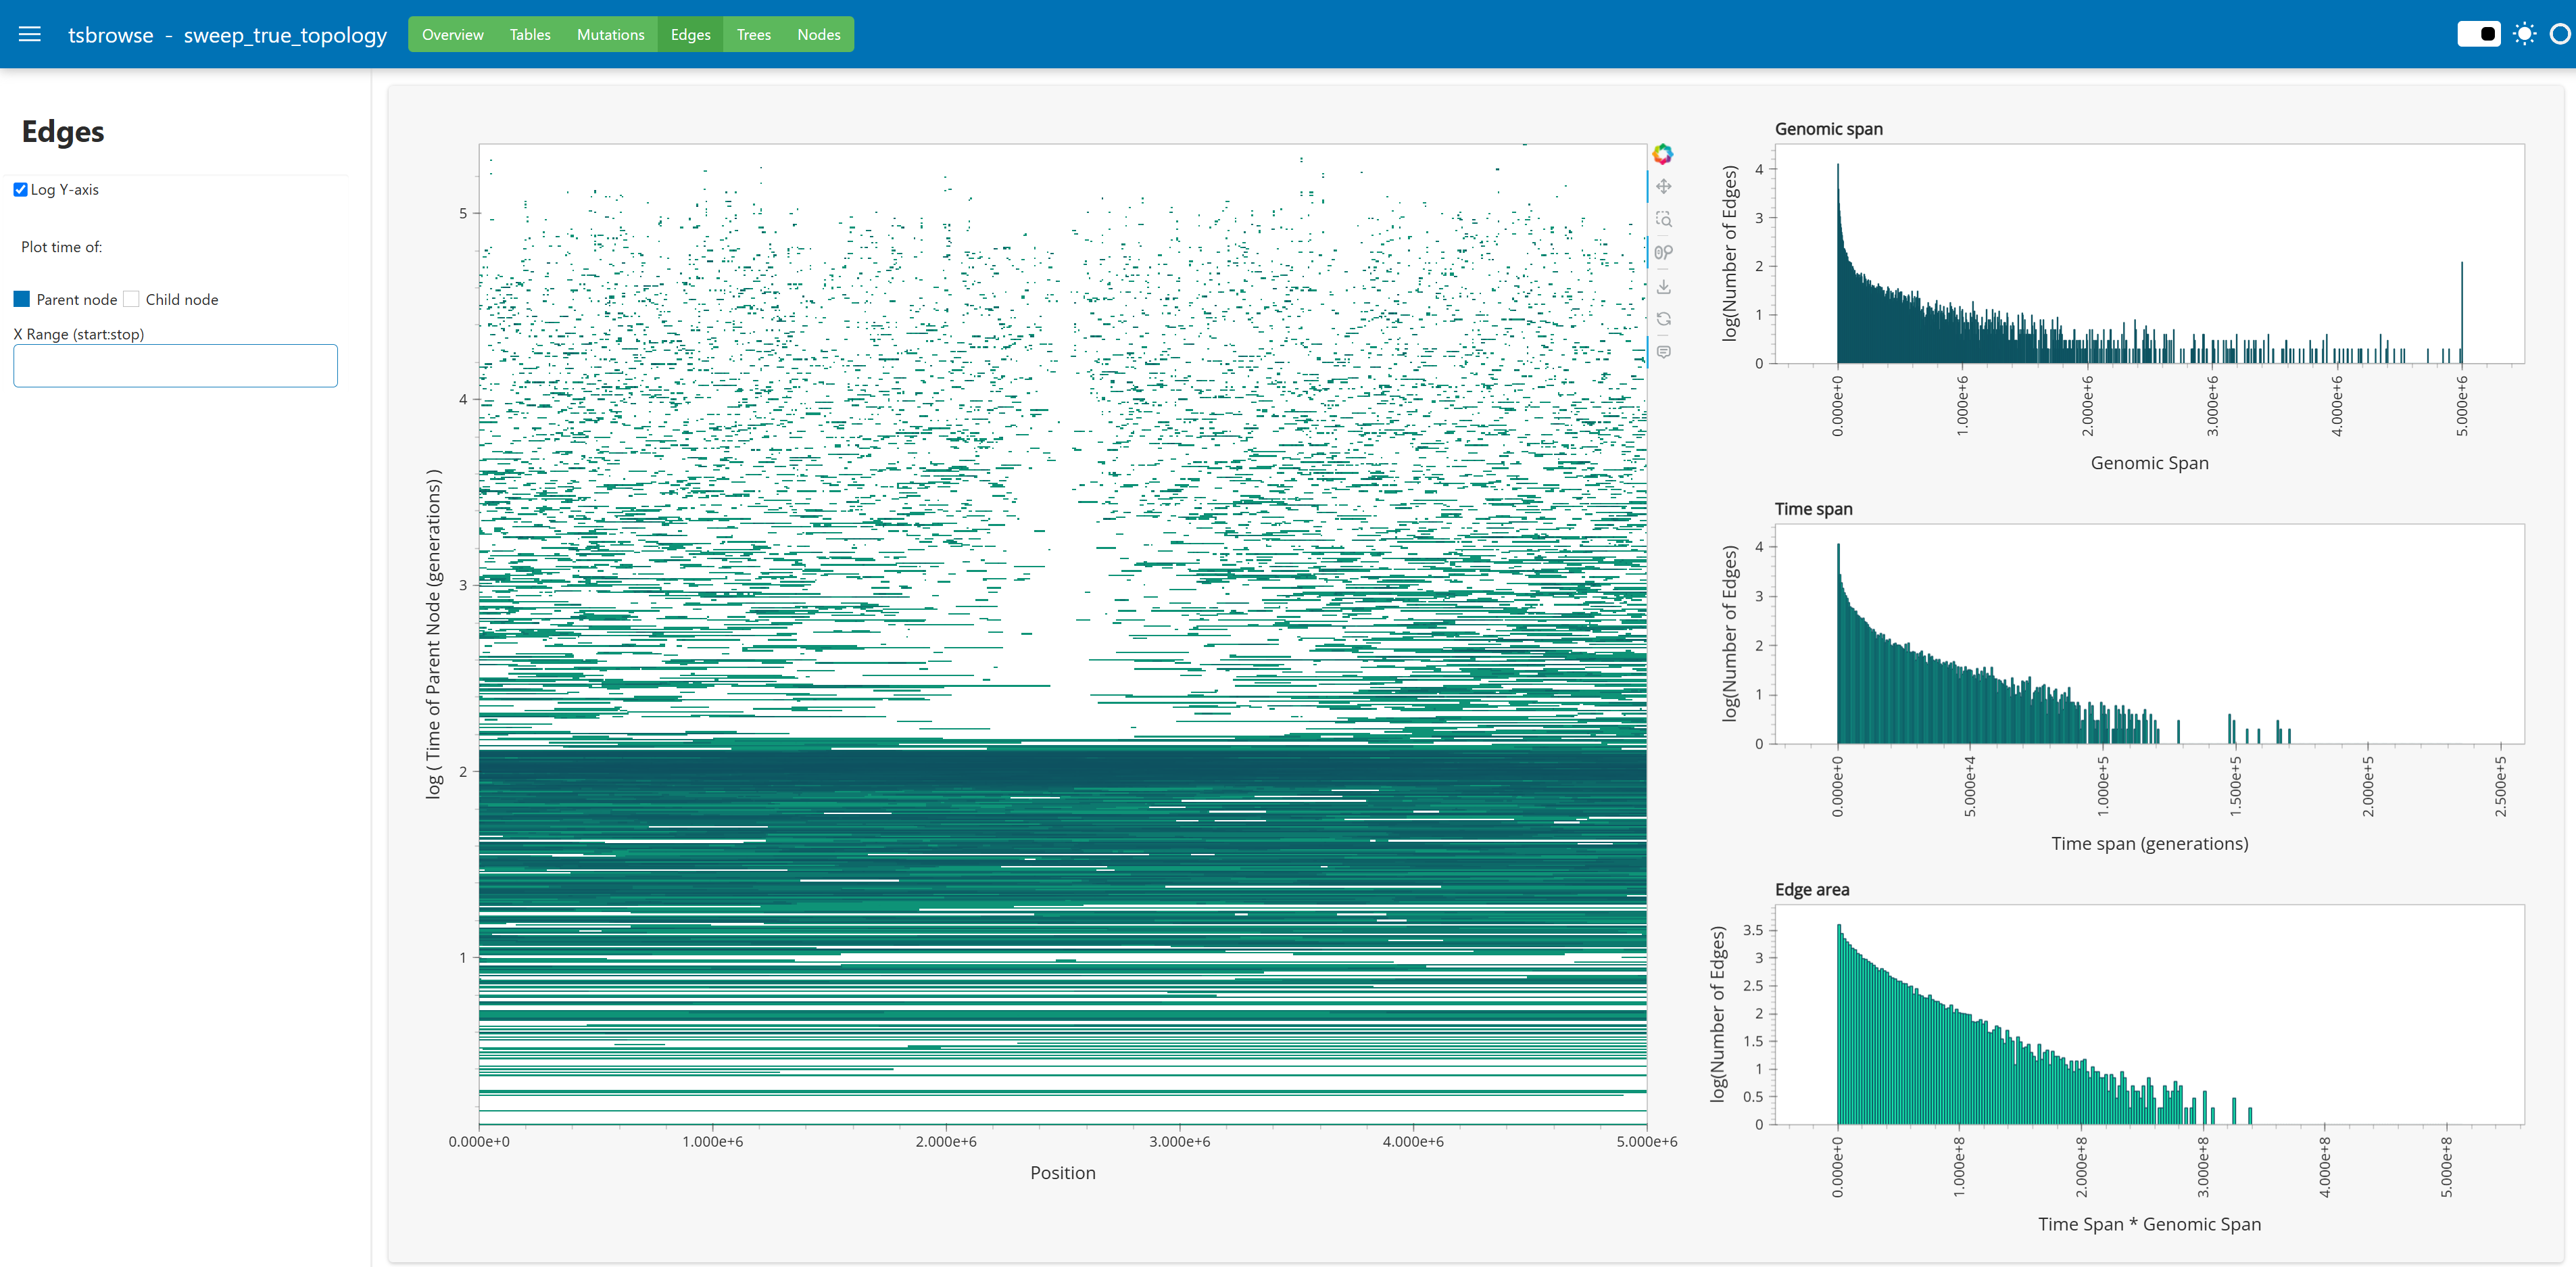
\includegraphics[width=0.95\linewidth]{figures/MainFig2.png}
    \caption{Screenshot of the Edges tab in \texttt{tsbrowse}.
        Visualisation of the edges in a simulated ARG with a strong selective
        sweep in the middle of the genome (see Supplement for details).
        Edges are shown in the main browser pane on the left, with additional
        histograms summarising the edges on the right.
        The effect of the sweep can be seen by the lack of edges crossing the
        centre of the simulated chromosome due to an excess of recent coalescent
        events. Moving away from the focal site, the oldest edges are the
        first to rejoin the ARG, followed by more recent edges, resulting in a
        wedge-like pattern of missing edges in the centre.
        \label{fig:Figure_2}}
\end{figure}
% \texttt{Tsbrowse}'s interface is built on the \texttt{Holoviz} ecosystem
% \citep{Holoviz}, which brings together \texttt{Datashader}, \texttt{Bokeh},
% \texttt{Panel}, \texttt{Holoviews} and other libraries to create seamless data
% visualisation pipelines even for large datasets. A key challenge with
% large-scale data visualisation is to maintain a responsive user interface.
% \texttt{Datashader} aggregates data and renders only the necessary data points
% at a given zoom level, thereby minimising the computational load on the
% browser. A \texttt{Bokeh} plotting back-end provides useful tools and widgets.
% The \textit{pan}, \textit{select} and \textit{zoom} tools enable interactivity
% with individual data points, allowing users to gain deeper insights from the
% data. The \texttt{serve} step accepts an optional input file containing
% sequence annotations. This allows users to overlay contextual information about
% genes or other sequence features. 
The user interface is presented as a dashboard, with pages to
describe various aspects of the ARG.
Figure~\ref{fig:Figure_2}
demonstrates the user interface using the Edges page as an example.
The plot on the left is an overview of the 33,929 edges
in a simulated ARG with a strong selective sweep (see
Sec.~\ref{subsec:sweep_simulation} for details).
Each edge is depicted as a horizontal line connecting the genomic coordinates
of the
parent and child nodes on the x-axis, and the y-axis shows the time of
either the parent or the child, as chosen by the user.
The user can interact with the main ``genome browser'' window
using a set of controls on the top-right corner (provided by Bokeh),
allowing the user to pan and zoom as required. The histograms to the
right then summarise the edges as depicted in the browser window.
A similar browser interface is provided for
nodes
(e.g. Fig~\ref{fig:Supplementary_Figure_3})
and mutations
(e.g. Fig~\ref{fig:Supplementary_Figure_4}).
\texttt{Tsbrowse} also provides an interactive table viewer with flexible
search and sorting utilities, which is a valuable debugging utility for
developers.

%The ability to explore ARG properties across the sequence and interact with the data makes the analysis of local genealogical patterns more intuitive.

\subsection{Applications}
The purpose of \texttt{tsbrowse} is to provide an interactive view of the
\texttt{tskit} ARG data model to guide intuition, improve inference quality
control and facilitate debugging. An example of how we can deepen our understanding
using the genome-browser-like perspective provided by \texttt{tsbrowse}
is given in the simulated ARG of Fig~\ref{fig:Figure_2}, where
the gap in the edges view corresponds to the characteristic dip in diversity
of a selective sweep. Comparing this ground truth to the ARGs inferred
by four different inference methods in Fig~\ref{fig:Supplementary_Figure_1},
we can see that there are substantial qualitative differences between the
results. These differences in ancestral haplotypes illustrated by
the edges view are unlikely to be captured by the tree-by-tree distance
metrics usually used to evaluate
inference methods~\citep[e.g.][]{kelleher2019inferring,zhang2023biobank},
providing further motivation for new and improved ways to compare
simulated and inferred ARGs~\citep{fritze2024forest}.

Interest in ARG-based methods is burgeoning, but the methods are new
and practical guidance on applying inferences to real data is lacking.
Data filtering is essential, and the effects of the
choices that must be made along any bioinformatics pipeline on the final
ARG are hard to predict and quantify. \texttt{Tsbrowse} was primarily
developed as a way to quickly visualise the effects of such filtering
choices on ARGs inferred by \texttt{tsinfer}, and it is now an indispensable
element of the inference pipeline. Fig~\ref{fig:Supplementary_Figure_2} 
shows a region of the 1000G data with gaps in site density that are spanned by
 exceptionally long edges, which are likely to bias downstream statistics.
These interactive visualisations have also helped diagnose issues with
the \texttt{tsinfer} inference algorithm.
Fig~\ref{fig:Supplementary_Figure_3} shows the genomic spans of
ancestral nodes in an ARG inferred with \texttt{tsinfer}, demonstrating a clear
excess of long haplotypes in the very ancient past. These insights
have helped guide development and
may lead to significant improvements in performance.

% . Population genetics theory predicts that IBD
% (Identical By Descent) segments break down over time, resulting in shorter
% ancestral segments further back in the history of the samples. At time,
% \textit{y \textgreater{0.8}}, the plot reveals a pattern of node spans contrary
% to this expectation. It confirms a known algorithmic artefact due to which
% disproportionately long old ancestors are generated.

% We demonstrate a further application of tsbrowse in validating inferences
% (Supplementary Figures 
% \ref{fig:Supplementary_Figure_3}). Supplementary Figure
% \ref{fig:Supplementary_Figure_2} shows how mutation patterns in a 2D plot of
% genomic position and mutation age are helpful in spotting poorly inferred
% regions. Excluding regions with low site density from the variant data improves
% the quality of inference (Panel B). 
% Supplementary Figure
% \ref{fig:Supplementary_Figure_3} shows the genomic spans of ancestral nodes in
% an ARG inferred with tsinfer. Population genetics theory predicts that IBD
% (Identical By Descent) segments break down over time, resulting in shorter
% ancestral segments further back in the history of the samples. At time,
% \textit{y \textgreater{0.8}}, the plot reveals a pattern of node spans contrary
% to this expectation. It confirms a known algorithmic artefact due to which
% disproportionately long old ancestors are generated.

% Supplementary Fig. \ref{fig:Supplementary_Figure_4}, a screenshot of the
% Mutations page for SARS-CoV-2 ARGs \citep{zhan2023towards} demonstrates
% tsbrowse's ability to handle diverse data sources. This plot represents a total
% of \textcolor{red}{X million} mutations from an inference of
% \textcolor{red}{1.27 million} sequences. After executing the
% \texttt{preprocess} step, the page loads in \textcolor{red}{X} seconds on a
% system with \textcolor{red}{Y GB RAM}, showing that it is possible to visualise
% large-scale datasets in a performant way. Panel B demonstrates a useful
% interactive feature; additional information about a mutation event (for
% example, the mutational frequency in predefined populations, or the number of
% sample nodes carrying the mutation) is displayed on mouse-over of individual
% data points.

\section{Discussion} \label{sec:Discussion}
Visualisation of tree topology is a central task in phylogenetics,
and although numerous tools
exist~\citep[e.g.][]{huson2007dendroscope,vaughan2017icytree},
the methods can typically only handle a few hundred nodes.
Visualisation of large-scale tree topologies with millions of nodes
requires much more sophisticated approaches
to capture topological features at different scales,
and is an active research area~\citep{wong2022dynamic,kramer2023treenome}.
Adapting such methods, and integrating into \texttt{tsbrowse} to provide
a local tree viewer that operates at the million-node scale
is an important direction for future work.
An interactive viewer for the entire ARG topology, capturing
semantic properties of the graph at a range of scales, is an even more
ambitious goal, and would be a major asset for the field.

% In current practice, simulated ARGs are used as ground-truth to validate
% inferences from empirical data
% \citep{Kelleher2019,Zhang2023,Speidel2019,Gunnarsson2024.08.31.610248}.
% Sophisticated techniques
% \citep{haller2019tree,baumdicker2022efficient,adrion2020community,lauterbur2023expanding} to simulate ARGs
% under complex, realistic demographic models \cite{Anderson-Trocme2023} now
% exist. However, models of simulation do not capture \textit{all} the nuances of
% population datasets. This results in a clear gap between ARG inference and
% application. \texttt{Tsbrowse} captures ARG properties in a model-free way,
% providing the means to qualitatively assess inferences. With notable features
% of browsability along the genome, scalability and applicability to diverse data
% sources, inference and simulation methods, \texttt{tsbrowse} has the potential
% to be integrated into biobank-scale data pipelines to improve ARG inference and
% analysis.

% \section*{Acknowledgments}
% \section*{Author contributions}
% \section*{Supplementary Data}
% Supplementary data are available at \textcolor{red}{Bioinformatics online}.
% \section*{Conflict of interest}
% No competing interest is declared.

\section*{Funding}
This work was supported by funding from the Biotechnology and Biological
Sciences Research Council (UKRI-BBSRC) [grant number BB/T008784/1],
\textcolor{red}{add Novo funding}. DMR is funded by 
a studentship from the Wellcome Programme in Genomic Medicine and Statistics.
JK acknowledges EPSRC (research grant EP/X024881/1),
NIH (research grants HG011395 and HG012473)
and the Robertson Foundation.

\bibliographystyle{natbib}
\bibliography{reference}

\clearpage \onecolumn \setcounter{figure}{0}
% Reset the figure counter
\renewcommand{\thefigure}{S\arabic{figure}}
% Change figure numbering to S1, S2, etc. 

\section{Supplementary Material}
\subsection{Simulation of truth dataset (Fig. \ref{fig:Figure_2})}
\label{subsec:sweep_simulation}
Ancestral
histories of 300 samples were simulated with \texttt{SweepGenicSelection}
function in \texttt{msprime (version 1.3.3)}. A combination of models was used:
in the recent past, a selective sweep was simulated with a beneficial allele
situated in the middle of a 5 Mb sequence. The frequency of the allele in the
population was set at 0.0001 at the beginning of the sweep. The allele fixed in
the population at a frequency of 0.9999. The strength of selection was set
using the selection coefficient, \textit{s = 0.25}. A time increment,
\textit{dt = 1e-6} was used to step through the sweep. Mutations were added to
the ARG at a rate of 1e-6. For simulating history before occurrence of the
sweep, a standard coalescent model (Hudson's algorithm \citep{Hudson1983}) was
used until coalescence was achieved.

\subsection{Inference of selective sweep dataset (Suppl. Fig.
    \ref{fig:Supplementary_Figure_1})} The following software were used to infer
ARGs from the truth dataset described above: \texttt{tsinfer version 0.3.3}
\citep{kelleher2019inferring}, \texttt{tsdate version 0.2.1}, 
\texttt{Relate version 1.2.2} \citep{speidel2019method}, 
\texttt{ARG-needle version 1.0.3} \citep{zhang2023biobank},
\texttt{SINGER version 0.1.8-beta} \citep{deng2024robust}.
For all
methods, the following parameters of inference were used: \textit{recombination
    rate = 1e-8}, \textit{mutation rate = 1e-8}, \textit{effective population size
    = 10,000}. Default values were used for all other inference parameters.

\subsection{Inference of 1000 Genomes dataset (Suppl. Fig.
\ref{fig:Supplementary_Figure_2}, Suppl. Fig.
\ref{fig:Supplementary_Figure_3})} The 1000 Genomes dataset was downloaded from
\texttt{\url{https://ftp.1000genomes.ebi.ac.uk/vol1/ftp/data_collections/1000G_2504_high_coverage/working/20220422_3202_phased_SNV_INDEL_SV/}}.
Ancestral fasta sequences for chromosomes 17 and 20 (GRCh38) were downloaded
from the Ensembl database. Inference was performed with a Snakemake pipeline
(\texttt{\url{https://github.com/benjeffery/tsinfer-snakemake/}}) using
\texttt{tsinfer version 0.3.3} for the long arms of chromosome 17 and 20 after
filtering out duplicate variant positions, variants with missing or low quality
ancestral allele, singletons, n-1-tons and n-2-tons. Only bi-allelic SNPs were
included for inference. For the inference in Suppl. Fig.
\ref{fig:Supplementary_Figure_2}, all genomic regions were included. For the
inference in Suppl. Fig. \ref{fig:Supplementary_Figure_3}, genomic regions with
a site density lesser than 5 per kb were discarded. For Suppl. Fig.
\ref{fig:Supplementary_Figure_2}, \texttt{tsdate version 0.2.1} was used to
estimate the age of ancestral nodes with \textit{mutation rate = 1.29e-8},
setting all other parameters to default values. 

\subsection{Inference of SARS-CoV-2 ARGs}
The ARG shown in Fig \ref{fig:Supplementary_Figure_4} was inferred with
\texttt{sc2ts}~\citep{zhang2023biobank} using the Viridian
dataset~\citep{hunt2024addressing}. It consists of
2,482,157 samples
2,689,054 nodes,
2,689,982 edges
and
1,923,169 mutations.
% Trees   348
% Sequence Length 29904.0
% Time Units  days
% Sample Nodes    2482157
% Total Size  1.5 GiB
% Table   Rows    Size    Has Metadata
% Edges   2689982 82.1 MiB
% Individuals 0   24 Bytes
% Migrations  0   8 Bytes
% Mutations   1923169 202.7 MiB
% Nodes   2689054 1.1 GiB
% Populations 0   8 Bytes
% Provenances 1131    1.7 MiB
% Sites   29803   3.1 MiB
Running \texttt{tsbrowse preprocess} on the input \texttt{tszip} file (113M)
required 2m19s time elapsed (15m15s CPU time) on an Intel Core(TM) i7-9700 CPU.
The resulting \texttt{.tsbrowse} file size was 130M.
% Preprocessing completed. You can now view with `python -m tsbrowse serve v1-beta1_2023-02-21.pp.md.il.ts.tsbrowse`

% real    2m19.028s
% user    15m15.049s
% sys     0m8.159s
% ```
% Sizes:
% ```
% $ ls -lh v1-beta1_2023-02-21.pp.md.il.ts.ts*
% -rw-rw-r-- 1 jk jk 130M Mar 27 15:08 v1-beta1_2023-02-21.pp.md.il.ts.tsbrowse
% -rw-r--r-- 1 jk jk 113M Mar 27 15:04 v1-beta1_2023-02-21.pp.md.il.ts.tsz
% ```

\subsection{} Code to recreate datasets and infer ARGs are available in an
accompanying repository:
\texttt{\url{https://github.com/savitakartik/tsbrowse-paper}}.

\clearpage
\section{Supplementary Figures}
\begin{figure}
    \centering
    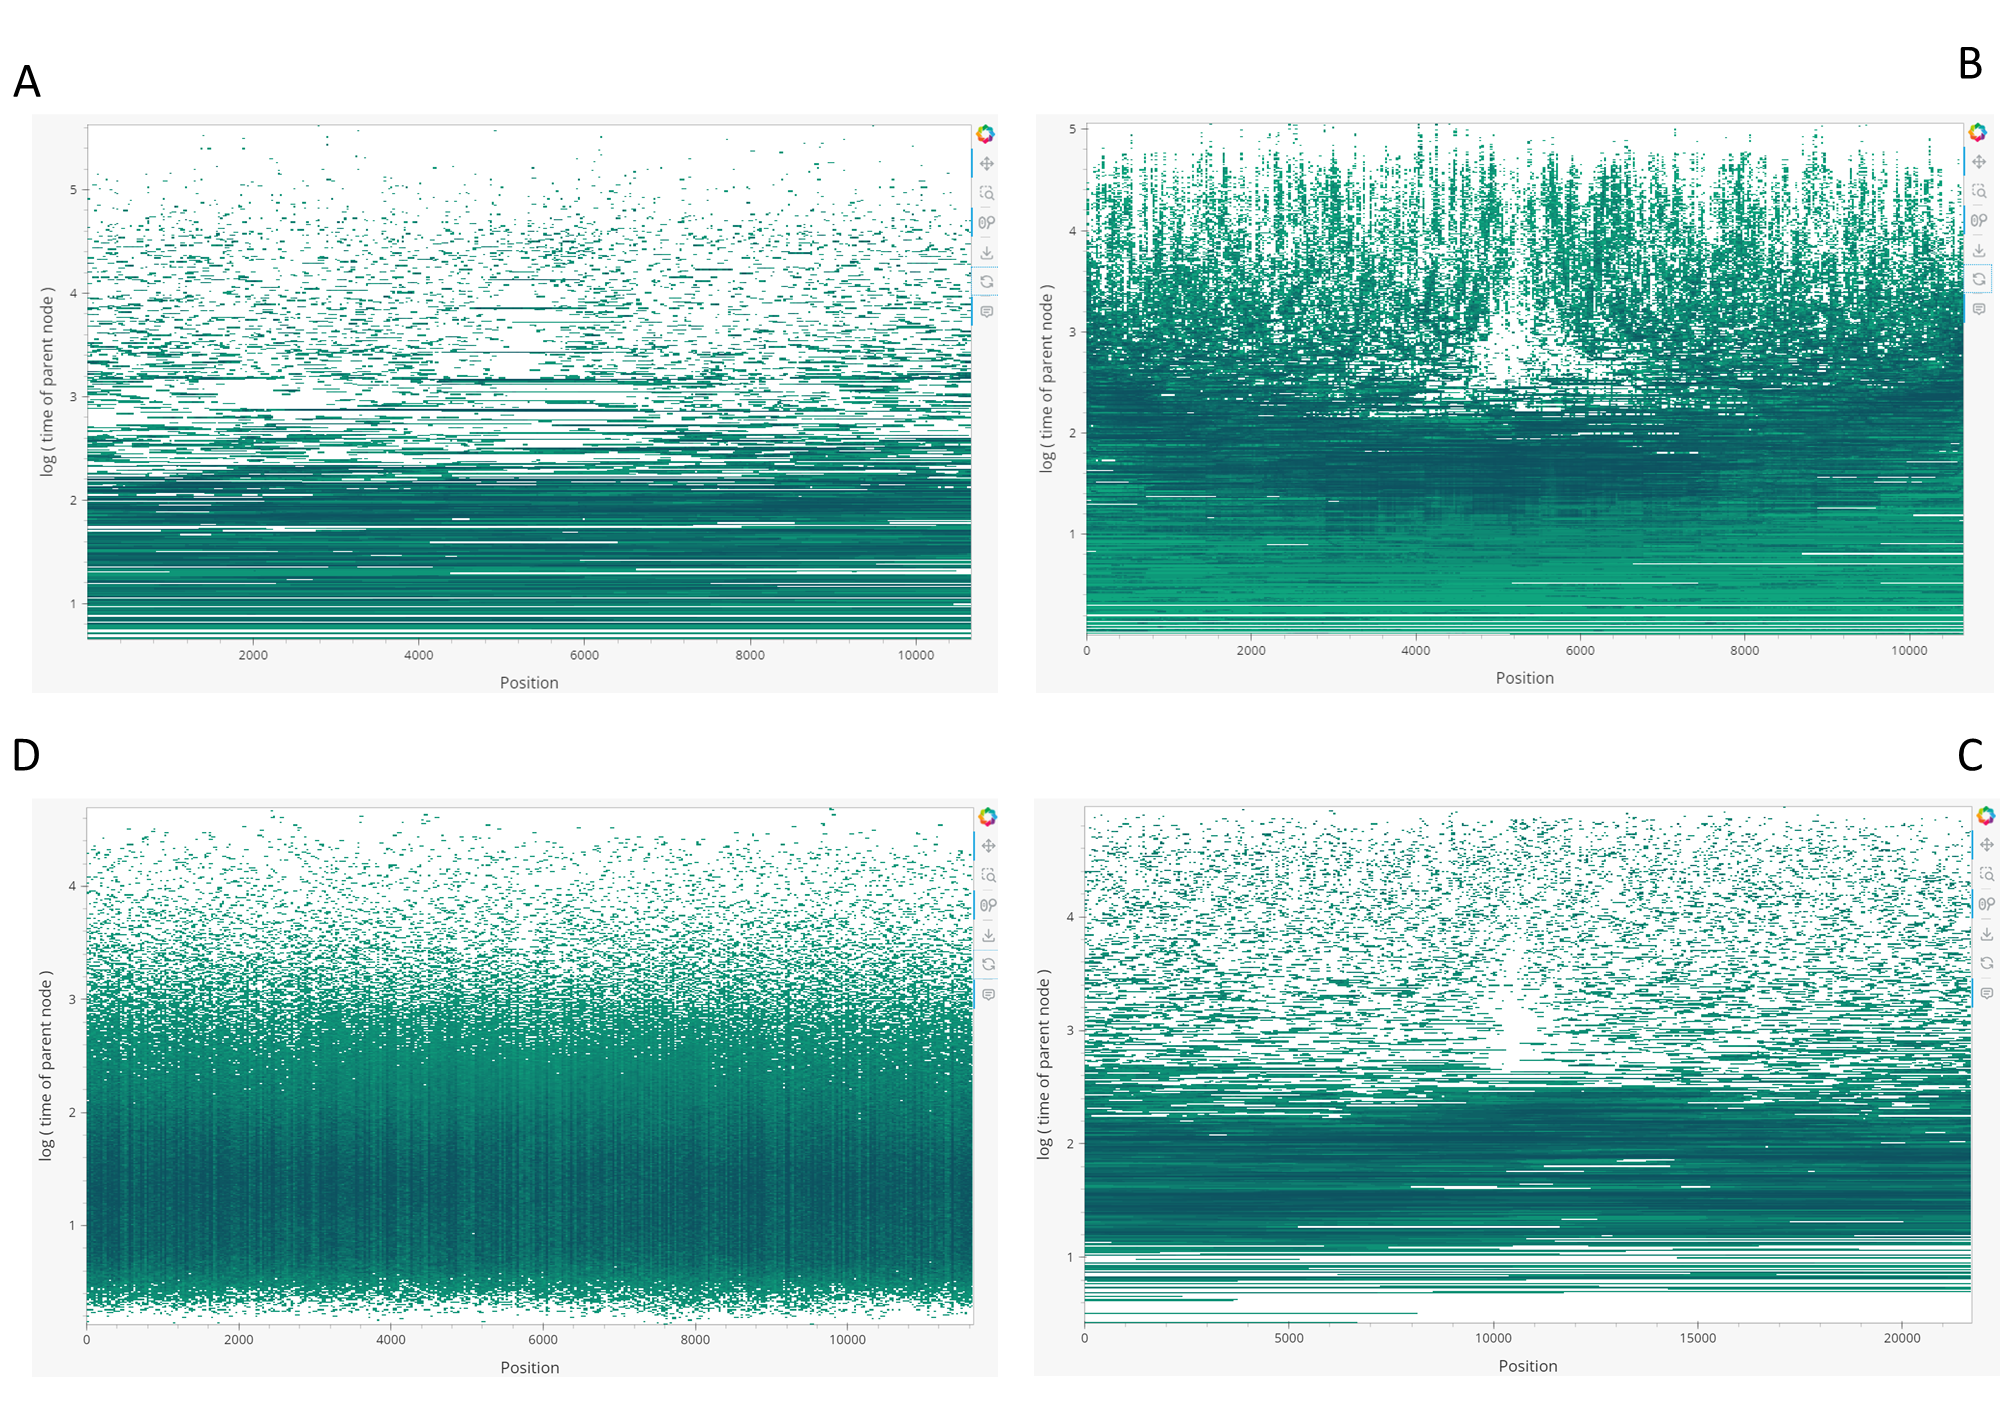
\includegraphics[width=0.95\linewidth]{figures/SuppFig1.png}
    \caption{\textbf{\texttt{tsbrowse} applied to inference methods}
    A screenshot of \texttt{tsbrowse}'s Edges view for tsinfer+tsdate (A),
ARG-Needle (B), Relate (C) and SINGER (D) inferences of the truth dataset
simulated under a selective sweep model (in Figure 2 of the main text). For
SINGER, an examplar ARG from the set of output posterior ARG samples is shown.
The X coordinate represents genomic position, each horizontal segment on the
plot shows the genomic coordinates that the edge spans, and Y coordinate shows
time of either the parent or child node in the edge.}
    \label{fig:Supplementary_Figure_1}
\end{figure}

\begin{figure}
    \centering
    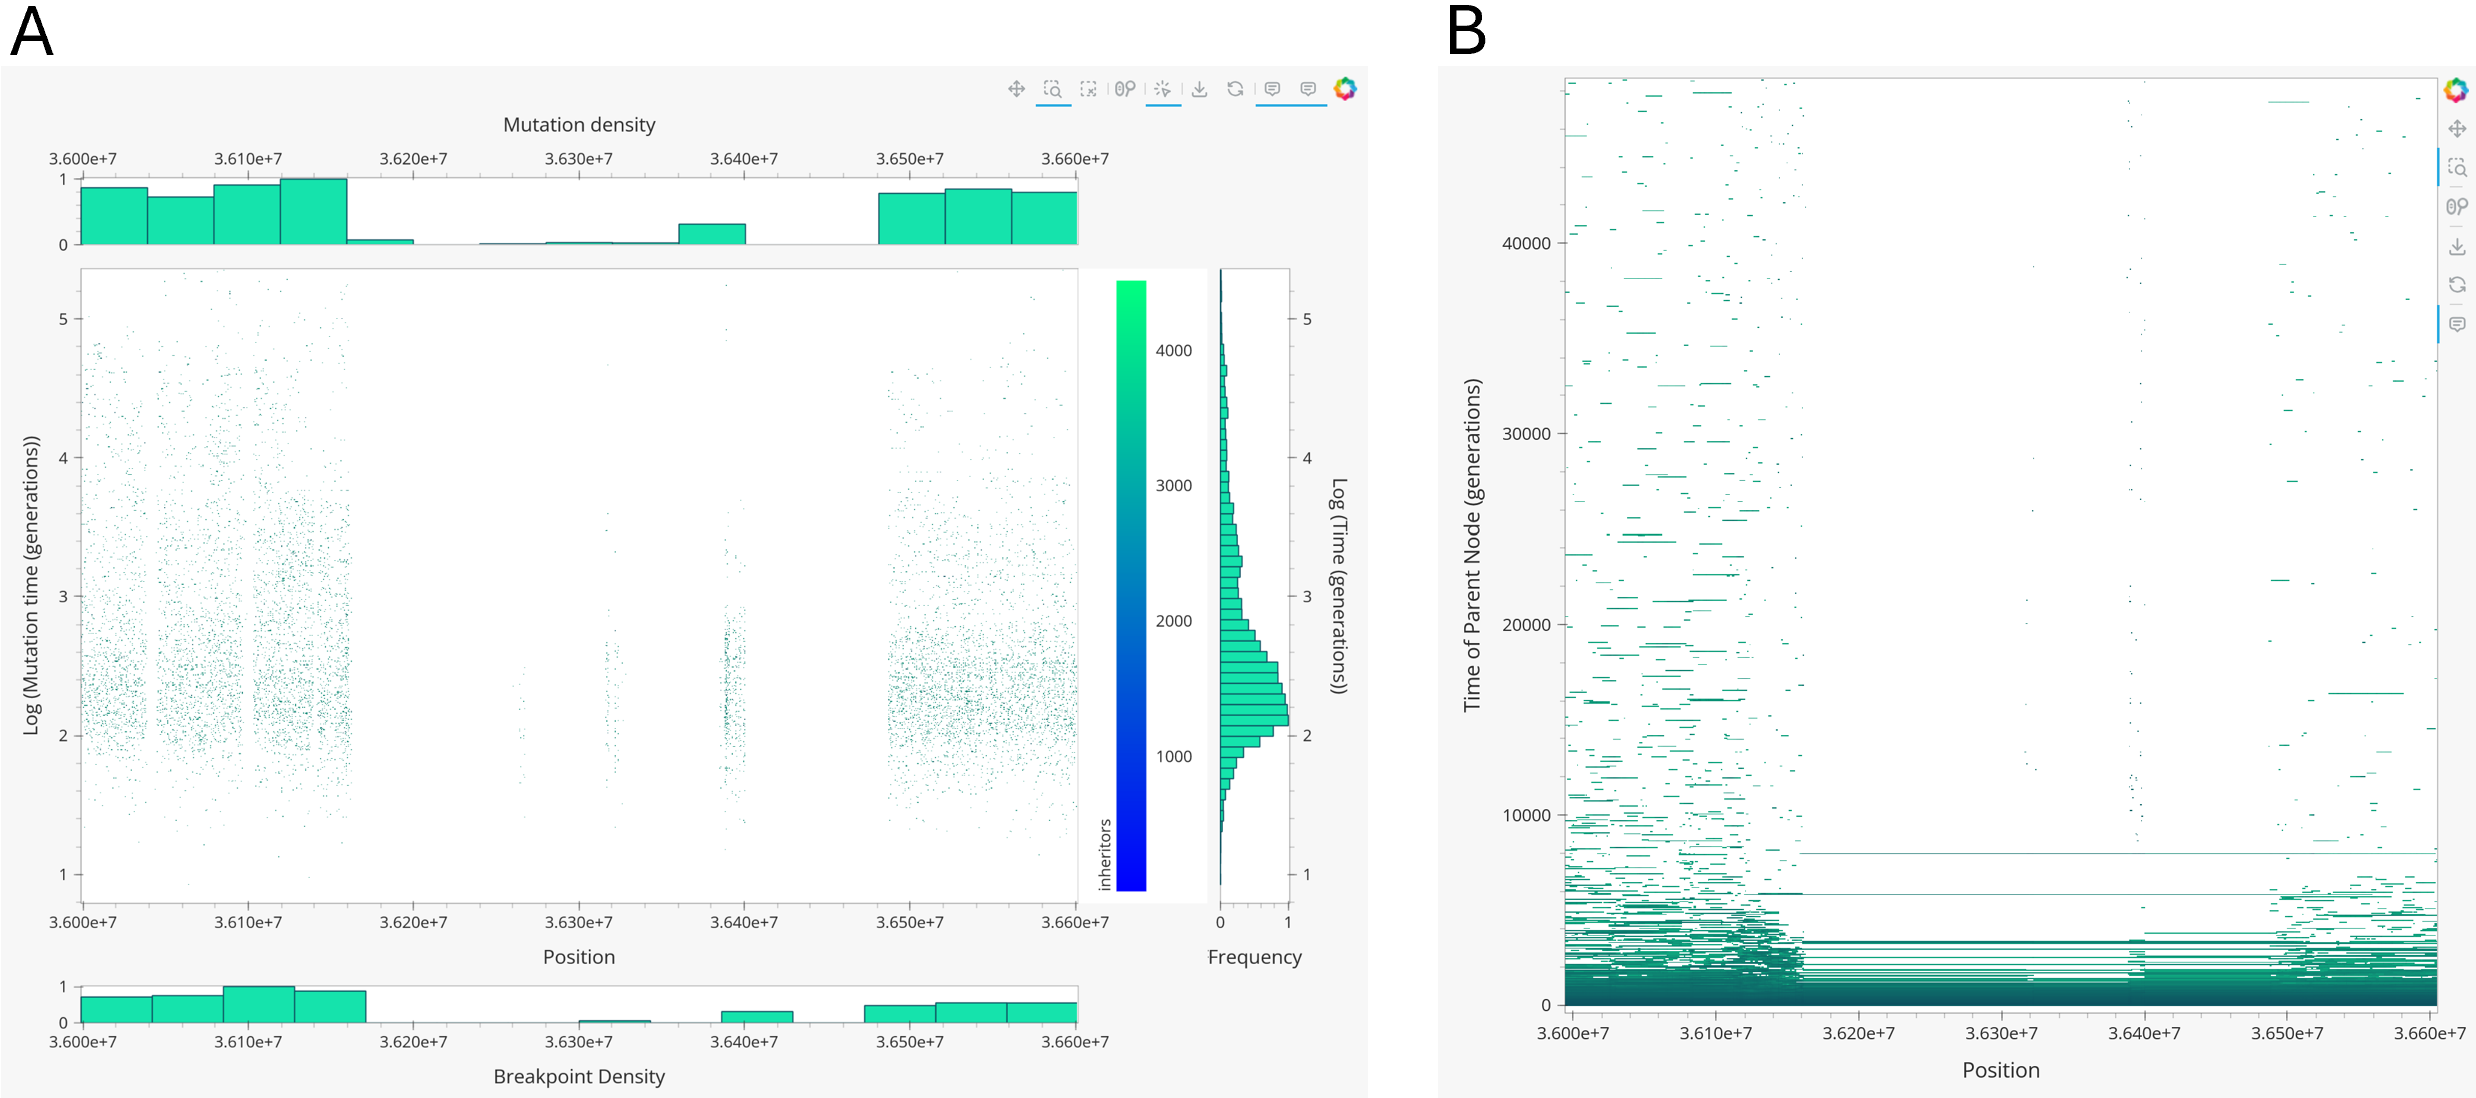
\includegraphics[width=0.95\linewidth]{figures/SuppFig2.png}
    \caption{\textbf{Identifying ARG inference problems with \texttt{tsbrowse}} 
Screenshots of \texttt{tsbrowse}'s Mutations view (A) and Edges view (B) for a
 600 kB region of chromosome 17 inferred from 3,202 participants from the 1000 
 Genomes Whole Genome Sequencing dataset (1000G) \citep{1000G2015, 1000GWGS}. 
 The poor performance of \texttt{tsinfer} in this variant-poor region is evidenced
  by the long edges spanning gaps in mutation density.}
    \label{fig:Supplementary_Figure_2}
\end{figure}

\begin{figure}
    \centering
    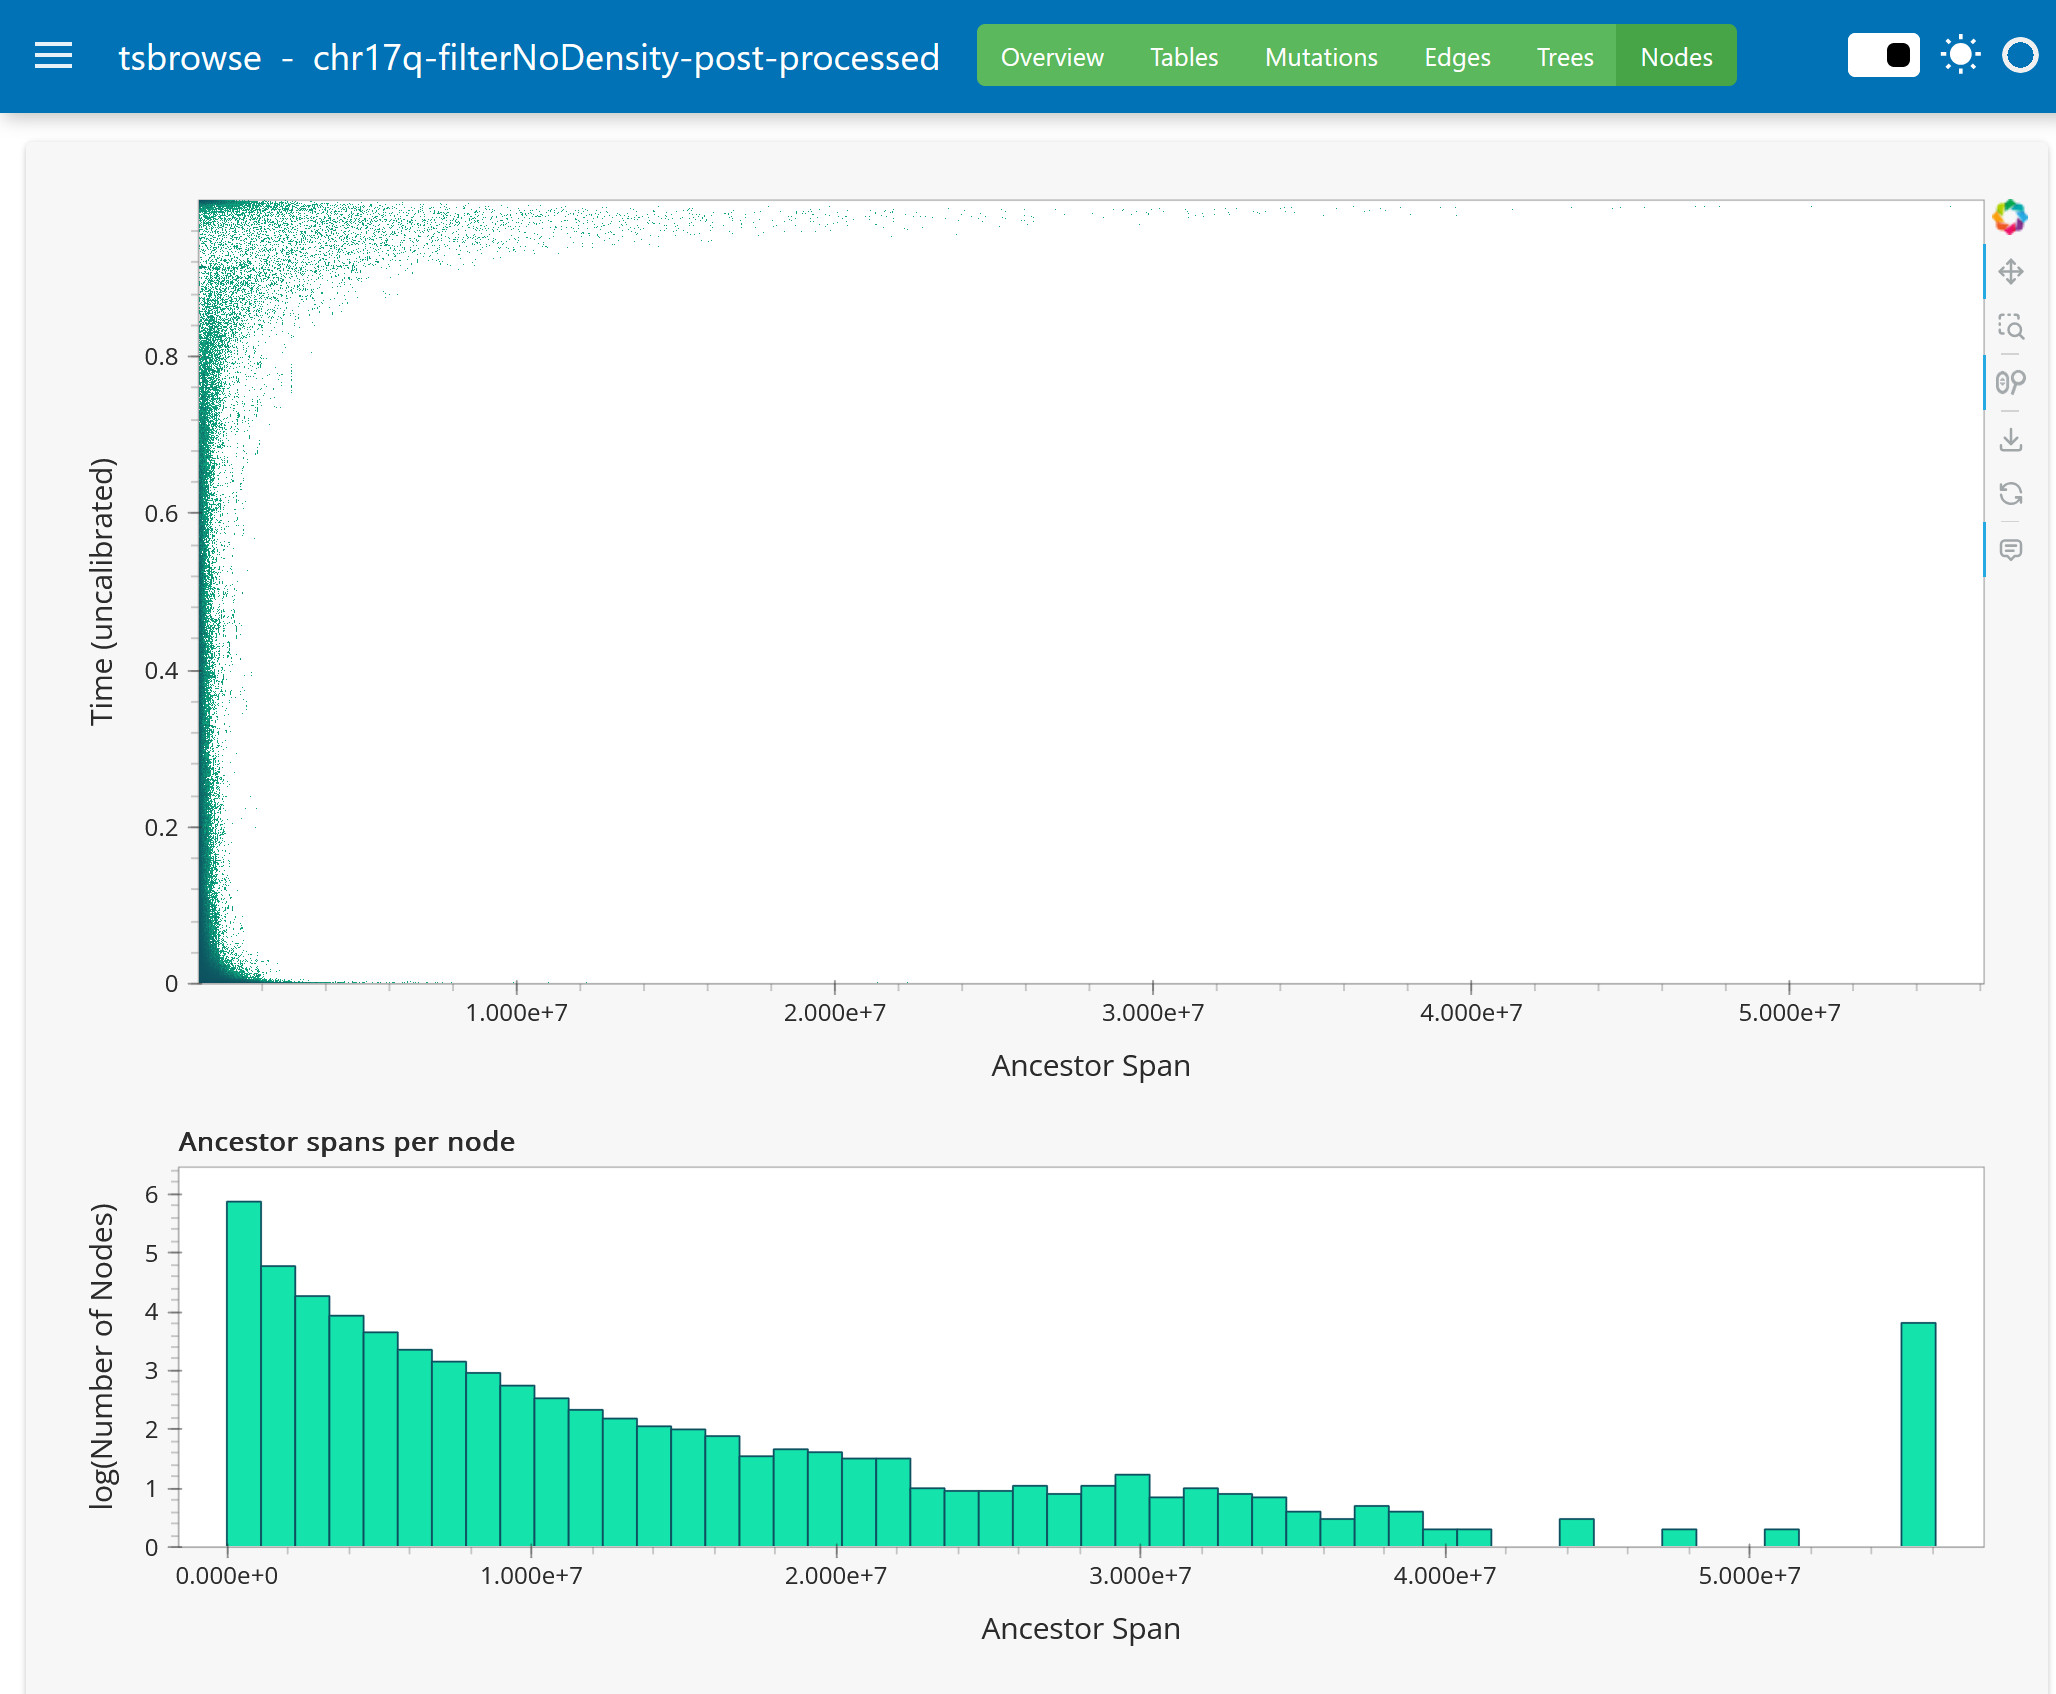
\includegraphics[width=0.95\linewidth]{figures/SuppFig3.png}
    \caption{\textbf{A view of the Nodes page for a 1000 Genomes inference.} A
        screenshot of \texttt{tsbrowse}'s Nodes view for an inference of the long arm
        of chromosome 20 from the 1000 Genomes whole-genome sequencing dataset. At the
        top is a plot of node spans over time. The length of sequence that the nodes
        span is shown on the X axis, and the time of nodes is shown on the Y axis. The
        histogram at the bottom shows the distribution of node spans. }
    \label{fig:Supplementary_Figure_3}
\end{figure}

\begin{figure}
    \centering
    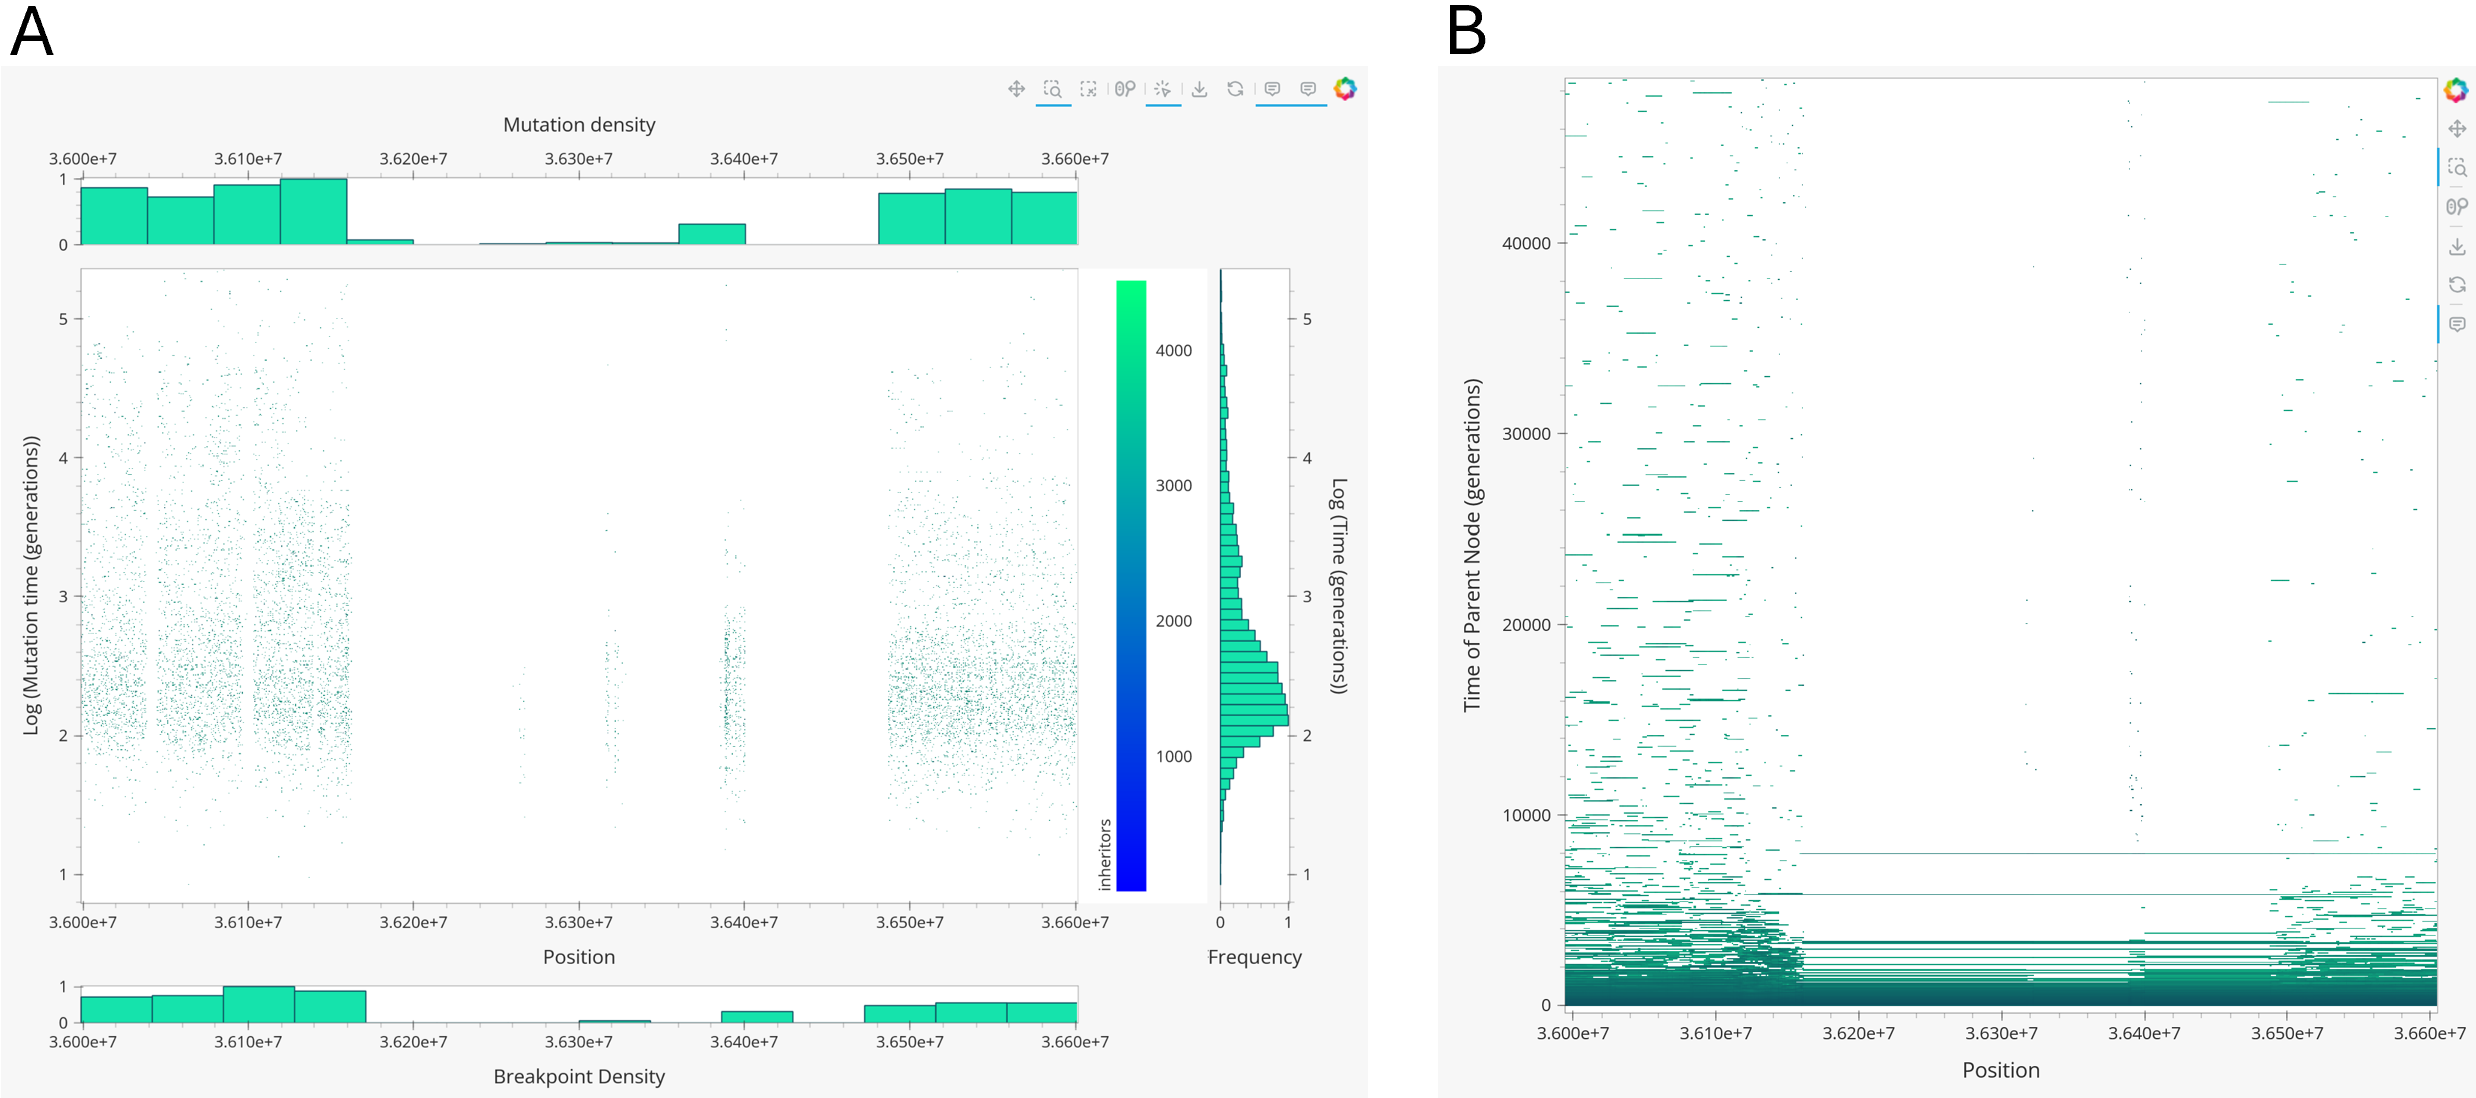
\includegraphics[width=0.95\linewidth]{figures/SuppFig4.png}
    \caption{\textbf{\texttt{tsbrowse} applied to SARS-CoV-2 ARGs.}
        A screenshot of \texttt{tsbrowse}'s depiction of
        1,923,169 mutations in an
        ARG inferred by \texttt{sc2ts}; see  text for details. Also shown are the
        gene annotations along the X-axis.}
    \label{fig:Supplementary_Figure_4}
\end{figure}
\end{document}
